\raggedbottom
\chapter{Databáze}

V této práci jsme využívali dvě databáze fotopletysmografických (\acs{PPG}) signálů: CapnoBase a \acl{BUT PPG} (BUT PPG).

Na těchto databázích jsme testovali a porovnávali výsledky použitých algoritmů.
U databáze CapnoBase jsme porovnávali naměřené systolické vrcholy s referenčními hodnotami a díky tomu jsme porovnávali i rozdíl v srdeční tepové frekvenci (\acs{TF}).
U databáze \acs{BUT PPG} nebyly referenční hodnoty systolických vrcholů k dispozici, ale byly zde referenční hodnoty \acs{TF} signálů a s nimi jsme porovnávali výsledky algoritmů.

\section{CapnoBase}

CapnoBase je veřejně dostupná databáze, která byla vytvořena primárně za účelem zkoumání respiračních a kardiovaskulárních parametrů z klinického prostředí.
Poskytuje záznamy obvykle dlouhé osm minut včetně \acs{PPG} a elektrokardiografických (EKG) signálů.
Jelikož jsou v této databázi u jednotlivých \acs{PPG} křivek k dispozici ručně označené referenční systolické vrcholy odvozené z EKG \cite{CapnoBase},
lze ji využít k přímému vyhodnocení úspěšnosti zvoleného algoritmu při detekci tepových komplexů i odhadu \acs{TF}.
Vzhledem k relativní délce a stabilitě záznamů vzniká prostor k testování robustních metod potlačení rušení či detekci \acs{TF} v různých, převážně nemocničních, situacích \cite{Karlen2013, Charlton2022}.
CapnoBase obsahuje údaje od 42 dětských a dospělých subjektů podstupujících plánovaný chirurgický zákrok a anestezii \cite{Charlton2022}.

\section{\acs{BUT PPG}}
Databáze \acs{BUT PPG} vznikla na Fakultě elektrotechniky a komunikačních technologií \acs{VUT} za účelem zkoumání kvality \acs{PPG} záznamů a odhadu \acs{TF}.
V nové rozšířené verzi obsahuje 3,888 desetisekundových měření od 50 dobrovolníků (25 žen a 25 mužů) ve věku 19 až 76 let, a to v klidu i při různých typech pohybových aktivit.
Záznamy byly pořízeny chytrými telefony (Xiaomi Mi9 a Huawei P20 Pro) se vzorkovací frekvencí 30 Hz, zatímco pro referenční EKG a akcelerometrická (ACC) data byl použit mobilní rekordér Bittium Faros 360 či 180 se vzorkovacími frekvencemi 1,000 Hz (EKG) a 100 Hz (ACC) \cite{BUT_PPG}.
Z videa byl extrahován průměr červené složky, který sloužil jako surový \acs{PPG} signál.
Postup je zobrazen na obrázku \ref{fig:videoZaznamPPG}.

Každý \acs{PPG} záznam byl synchronizován s ECG a rozdělen do desetisekundových segmentů, které následně hodnotili tři až pět expertů.
Pro označení kvality vycházeli výhradně z rozdílu mezi \acs{TF} odhadnutou z \acs{PPG} a referenční tepovou frekvencí z EKG.
Pokud byla odchylka do pěti úderů za minutu, bylo dané měření označeno jako „dobré“ (1), jinak jako „špatné“ (0)
Tato hranice vychází z mezinárodní normy IEC 60601-2-27 a v databázi \acs{BUT PPG} je aplikována ještě přísněji \cite{BUT_PPG}.
Přibližně polovina záznamů vznikla přiložením prstu na zadní kameru a LED, druhá pak snímáním ucha v poloze připomínající telefonování.
V novější části databáze se rozšiřuje množství subjektů i situací, včetně manipulací s osvětlením, vyšším tlakem prstu na čočku, mluvením či chůzí, a nově se přidávají i údaje o krevním tlaku, glykémii a saturaci krve kyslíkem.
Díky této variabilitě podmínek a bohatým anotacím je \acs{BUT PPG} unikátním zdrojem pro testování robustnosti algoritmů detekce \acs{TF} a pro posuzování použitelnosti krátkých PPG signálů z mobilního telefonu v reálné praxi.

\begin{figure}[ht]
	\centering
	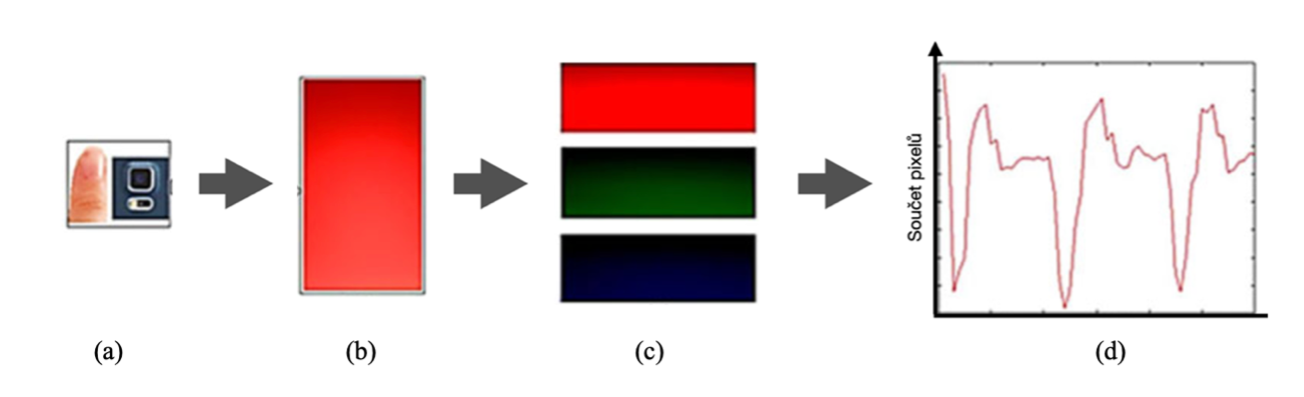
\includegraphics[width=0.8\textwidth]{./obrazky/videoZaznamPPG.png}
	\caption[Získání PPG signálu pro databázi \acs{BUT PPG}]{Záznam videa na kameru mobilního telefonu (a), jeden vybraný snímek ze záznamu (b), snímek rozložen na tři barevné složky (c), PPG signál vykreslený z červené složky (d), upraveno z \cite{Siddiqui2016}.}
	\label{fig:videoZaznamPPG}
\end{figure}

Spojením klinicky orientované databáze CapnoBase a mobilně zaměřené \acs{BUT PPG} vzniká možnost vzájemného porovnání a ověření přesnosti metod,
které musejí obstát v rozdílných kontextech: v relativně stabilním operačním prostředí a v krátkých záznamech z chytrého telefonu.